\documentclass[namecite, fleqn]{goose-article}

\usepackage{framed}

\title{Simo elasto-plastic model for finite strains}

\author{Tom W.J.\ de Geus}

\hypersetup{pdfauthor={T.W.J. de Geus}}

\newcommand\leftstar[1]{\hspace*{-.3em}~^\star\!#1}
\newcommand\ST[1]{\hspace*{-.3em}~^\star\!#1}

\newcommand\T[1]{\bm{{#1}}}

\newcommand\TT[1]{\mathbb{{#1}}}

\begin{document}

\maketitle

\section{Model}

This document is based on the work by \citet{Geers2004},
who presented this model extended with damage.

\paragraph{Key tensors}

\begin{itemize}

    \item \emph{Finger tensor} (also known by the name \emph{left Cauchy-Green deformation})
    \begin{equation}
        \T{b} \equiv \T{F} \cdot \T{F}^T
    \end{equation}

    \item \emph{Left stretch tensor}:
    \begin{equation}
        \T{v} \equiv \sqrt{\T{b}}
    \end{equation}

    \item \emph{Hencky’s logarithmic strain tensor}:
    \begin{equation}
        \T{\varepsilon} \equiv \ln \T{v} = \tfrac{1}{2} \ln \T{b}
    \end{equation}

    \item \emph{Kirchhoff stress tensor} $\T{\tau}$, which is related to the
    \emph{Cauchy stress tensor} $\T{\sigma}$ as follows:
    \begin{equation}
        \T{\tau} \equiv J \T{\sigma}
    \end{equation}
    where $J$ is the volume change ratio
    \begin{equation}
        J \equiv \det \T{F}
    \end{equation}

\end{itemize}

\paragraph{Model}

This model relies on splitting the deformation gradient $\T{F}$ in an elastic part,
$\T{F}_\mathrm{e}$, and a plastic part, $\T{F}_\mathrm{p}$, as follows:
\begin{equation}
    \T{F} \equiv \T{F}_\mathrm{e} \cdot \T{F}_\mathrm{p}
\end{equation}
The model is fully defined in the deformed configuration.
To that end it is defined in terms of
the logarithmic strain.
The Kirchhoff stress $\T{\tau}$ is thereby related to the
logarithmic elastic strain $\T{\varepsilon}_\mathrm{e} \equiv \tfrac{1}{2} \ln \T{b}_\mathrm{e}$
in the usual way:
\begin{equation}
    \T{\tau} \equiv K \mathrm{tr} \left( \T{\varepsilon}_\mathrm{e} \right) \T{I}
    + 2 G \T{\varepsilon}_\mathrm{e}^\mathrm{d}
\end{equation}
where $K$ is the bulk modulus and $G$ is the shear modulus,
$\T{I}$ is the second-order unit tensor,
and $\T{\varepsilon}_\mathrm{e}^\mathrm{d}$ is the deviator of the elastic strain tensor.
Equivalently this can be expressed in terms of a fourth order material stiffness
\begin{equation}
    \T{\tau} \equiv \TT{C} : \T{\varepsilon}_\mathrm{e},
    \quad
    \TT{C}_\mathrm{e} = K \T{I} \otimes \T{I} + 2 G \TT{I}^\mathrm{d}
    \label{eq:tangent:elas}
\end{equation}
where the fourth order tensor $\TT{I}^\mathrm{d} = \TT{I} - \tfrac{1}{3} \T{I} \otimes \T{I}$
projects an arbitrary tensor on its deviator part
($\TT{I}^\mathrm{d} : \T{A} \equiv \T{A}^\mathrm{d}$).
The elastic domain is bounded by a yield function, that,
following standard $J_2$ plasticity, reads
\begin{equation}
    \Phi(\T{\tau}, \varepsilon_\mathrm{p}) \equiv \tau_\mathrm{eq}
    - \tau_\mathrm{y}(\varepsilon_\mathrm{p}) \leq 0
\end{equation}
where
\begin{equation}
    \tau_\mathrm{eq} \equiv \sqrt{ \T{\tau}^\mathrm{d} : \T{\tau}^\mathrm{d} }
\end{equation}
is the equivalent stress; $\tau_\mathrm{y}$ is the equivalent yield stress that may,
in the case of hardening, be a function of the effective plastic strain $\varepsilon_\mathrm{p}$.
The latter depends on the entire strain history:
\begin{equation}
    \varepsilon_\mathrm{p} = \int\limits_0^t \dot{\gamma} \;\mathrm{d}t^\prime
    \label{eq:history}
\end{equation}
whereby the plastic strain rate, $\dot{\gamma}$, is by construction nonnegative.
Also note that it is defined in terms of some pseudo-time, as there is no rate sensitivity.
In line with $J_2$-plasticity, normality is used to determine the direction of plastic flow.
This corresponds to the following associative flow rule:
\begin{equation}
    \dot{\bm{\varepsilon}}_\mathrm{p} = \dot{\gamma} \bm{N}
    \label{eq:flow-rule}
\end{equation}
where $\bm{N}$ is the Prandtl-Reuss flow vector, which is defined through normality:
\begin{equation}
    \bm{N}
    = \frac{\partial \Phi}{\partial \T{\tau}}
    = \frac{3}{2} \frac{\T{\tau}^\mathrm{d}}{\tau_\mathrm{eq}}
\end{equation}

\paragraph{Trial state}

The path-dependent model is solved by discretising in pseudo-time.
Accordingly, the deformation is applied in small steps, transforming \cref{eq:history} in
\begin{equation}
    \varepsilon_\mathrm{p} = \sum \Delta \gamma^t
\end{equation}
Solving proceeds through the formulation of a trial state,
whereby the full deformation increment is assumed elastic.
From this potentially non-physical state one looks for the increment in plastic strain
that gives rise to a physically admissible state.

In particular, the incremental deformation tensor
\begin{equation}
    \T{f} = \T{F}^{t + \Delta t} \cdot \left[ \T{F}^t \right]^{-1}
\end{equation}
is used to define the trial state
\begin{equation}
    \begin{cases}
        \ST{\T{b}}_\mathrm{e} = \T{f} \cdot \T{b}_\mathrm{e}^t \cdot \T{f}^\mathsf{T}
        \\
        \ST{\varepsilon_\mathrm{p}} = \varepsilon_\mathrm{p}^t
    \end{cases}
\end{equation}
which gives rise to some $\ST{\T{\tau}}$ and corresponding $\ST{\tau}_\mathrm{eq}$ and $\ST{\T{N}}$.
The trial value for the yield function follows as:
\begin{equation}
    \ST{\Phi} = \ST{\tau}_\mathrm{eq} - \tau_\mathrm{y}(\ST{\varepsilon}_\mathrm{p})
\end{equation}
For any $\ST{\Phi} \leq 0$ the trial state is simply the physical admissible state.
Otherwise one has to look for a $\Delta \gamma$ such that
$\Phi(\T{\tau},\varepsilon_\mathrm{p}) = 0$.

\paragraph{Return mapping}

Given the plastic strain update $\Delta \gamma$ (whose value will be specified below),
following \cref{eq:flow-rule} the actual elastic strain
\begin{equation}
    \T{\varepsilon}_\mathrm{e} = \ST{\T{\varepsilon}}_\mathrm{e} - \Delta \gamma \,\ST{\T{N}}
\end{equation}
(here and below the superscript $t + \Delta t$ have been dropped,
which is trusted not to give confusion).
Consequently the stress reads
\begin{equation}
    \T{\tau} = \ST{\T{\tau}} - 2 G \Delta \gamma \, \ST{\T{N}}
\end{equation}
which, by construction, only affects the deviatoric part of $\T{\tau}$.
The stress deviator can be alternatively expressed as
\begin{equation}
    \T{\tau}^\mathrm{d}
    = \ST{\T{\tau}}^\mathrm{d}
    - 3 G \Delta \gamma \frac{\ST{\T{\tau}}^\mathrm{d}}{\ST{\tau}_\mathrm{eq}}
    = \left( 1 - \frac{3 G \Delta \gamma }{\ST{\tau}_\mathrm{eq}} \right) \ST{\T{\tau}}^\mathrm{d}
\end{equation}
from which the following expression for the equivalent stress can be expressed:
\begin{equation}
    \tau_\mathrm{eq} = \ST{\tau}_\mathrm{eq} - 3 G \Delta \gamma
\end{equation}
It can now be realised that the trial and updated deviatoric stresses are \emph{co-linear}:
\begin{equation}
    \frac{ \T{\tau}_\mathrm{d} }{ \tau_\mathrm{eq} }
    =
    \frac{ \ST{\T{\tau}}_\mathrm{d} }{ \ST{\tau}_\mathrm{eq} }, \quad
    \T{N} = \ST{\T{N}}
\end{equation}

To summarise, the return map involves:
\begin{equation}
    \begin{cases}
        \T{\tau} = \ST{\T{\tau}} - 2 G \Delta \gamma \T{N}
        \\
        \tau_\mathrm{eq} = \ST{\tau}_\mathrm{eq} - 3 G \Delta \gamma
        \\
        \varepsilon_\mathrm{p} = \ST{\varepsilon}_\mathrm{p} + \Delta \gamma
    \end{cases}
\end{equation}
The plastic strain update $\Delta \gamma$ follows from enforcing the yield function:
\begin{equation}
    \Phi(\T{\tau}, \varepsilon_\mathrm{p})
    = \ST{\tau}_\mathrm{eq}
    - 3 G \Delta \gamma - \tau_\mathrm{y} ( \ST{\varepsilon}_\mathrm{p} + \Delta \gamma ) = 0
    \label{eq:return-map:yield-function}
\end{equation}

\paragraph{Linear hardening}

Linear hardening corresponds to the following evolution of yield stress:
\begin{equation}
    \tau_\mathrm{y} ( \varepsilon_\mathrm{p} )
    = \tau_\mathrm{y0} + H \varepsilon_\mathrm{p}
\end{equation}
In this case, enforcing the yield function (as in
\cref{eq:return-map:yield-function}) corresponds to:
\begin{equation}
    \ST{\Phi} - 3 G \Delta \gamma + H \Delta \gamma = 0
\end{equation}
Solving for $\Delta \gamma$ results in
\begin{equation}
    \Delta \gamma = \frac{\ST{\Phi}}{H + 3G}
\end{equation}

\begin{framed}
\begin{quote}
    Note that although the model is defined in terms of the Kirchhoff stress $\T{\tau}$,
    the implementation outputs the Cauchy stress $\T{\sigma} = \T{\tau} / J$
    for convenience in use with Finite Elements.
    See below.
\end{quote}
\end{framed}

\section{Tangent}

\paragraph{Basic definition}

The consistent tangent operator, defined in the current configuration, is of the form
\begin{equation}
    \delta \bm{\tau}
    =
    \TT{K}_{(i)}
    : \T{L}_\delta^T
    =
    \TT{K}_{(i)}
    : \T{F}_{(i)}^{-T} \cdot \delta \T{F}^T
    \label{eq:tangent}
\end{equation}
where
\begin{equation}
    \bm{L}_\delta
    \equiv \delta \bm{F} \cdot \bm{F}_{(i)}^{-1}
    = \left( \bm{F}_{(i)}^{-T} \cdot \delta \bm{F}^T \right)^T
\end{equation}

\paragraph{Finite element formulation}

Starting from the strong from of the balance of linear momentum,
\begin{equation}
    \vec{\nabla} \cdot \T{\sigma}(\vec{x}) = \vec{0} \quad \forall \vec{x} \in \Omega
\end{equation}
in the Finite Element Method the problem is treated in its weak form.
In the absence of boundary tractions (e.g.\ for periodic boundary conditions), it reads:
\begin{equation}
    \int\limits_{\Omega} \big( \vec{\nabla} w )^T : \T{\tau} \frac{1}{J} d\Omega = 0
\end{equation}
which must hold for any possible test function $w(\vec{x})$.
Its solution is usually found by making use of consistent linearisation.
This corresponds to:
\begin{equation}
    \int\limits_{\Omega} \big( \vec{\nabla} w )^T
    : \TT{K}_{(i)}
    : \T{L}_\delta^T \frac{1}{J_{(i)}} d\Omega
    =
    - \int\limits_{\Omega} \big( \vec{\nabla} w )^T
    : \T{\tau}_{(i)} \frac{1}{J_{(i)}} d\Omega
\end{equation}


\begin{framed}
\begin{quote}
    It should now be obvious why the implementation outputs the Cauchy stress
    $\T{\sigma} = \T{\tau} / J$ and $(\TT{K}) / J$.
\end{quote}
\end{framed}

\paragraph{Details}

The tangent is composed of the linearisation of geometrical and material non-linearity, as follows:
\begin{equation}
    \TT{K} = \TT{K}_\mathrm{geo} + \TT{K}_\mathrm{mat}
\end{equation}
where the linearisation of geometrical non-linearity leads to:
\begin{equation}
    \TT{K}_\mathrm{geo} = - \TT{I}^\mathrm{RT} \cdot \T{\tau}
\end{equation}
and that of material non-linearity to:
\begin{equation}
    \TT{K}_\mathrm{mat}
    = \TT{C}
    : \frac{\partial \ST{\T{\varepsilon}}_\mathrm{e}}{\partial \ln \ST{\T{b}}_\mathrm{e}}
    : \frac{\partial \ln \ST{\T{b}}_\mathrm{e}}{\partial \ST{\T{b}}_\mathrm{e}}
    : \frac{\partial \ST{\T{b}}_\mathrm{e}}{\partial \T{L}_\delta^T}
\end{equation}
whereby the different constituents are:
\begin{itemize}

    \item The derivative of the constitutive response:
    \begin{equation}
        \TT{C} =
        \begin{cases}
            \TT{C}_\mathrm{e} \quad\mathrm{if}\; \phi \leq 0 \\
            \TT{C}_\mathrm{ep} \quad\mathrm{otherwise}
        \end{cases}
    \end{equation}
    where $\TT{C}_\mathrm{e}$ is defined in \cref{eq:tangent:elas}, and
    \begin{align}
        2 \; \TT{C}_\mathrm{ep}
        &= \left[
            a_0 \T{I} \otimes \T{I}
            + (1 - 3 a_0) \TT{I}^s - 2 (a_0 - a_1) \ST{\T{N}} \otimes \ST{\T{N}}
        \right] : \TT{C}_\mathrm{e}
        \\
        &= \left( \frac{K}{2} - \frac{G}{3} + a_0 G \right) \T{I} \otimes \T{I}
        + (1 - 3 a_0) G \TT{I}^s + 2 (a_0 - a_1) \ST{\T{N}} \otimes \ST{\T{N}}
    \end{align}
    where
    \begin{equation}
        a_0 = \frac{\Delta \gamma G}{\ST{\tau}_\mathrm{eq}}
        \qquad
        a_1 = \frac{G}{\frac{\partial h}{\partial \varepsilon_\mathrm{p}} + 3 G}
    \end{equation}

    \item The derivative of Hencky’s strain with respect to the logarithm
    of the Finger tensor is simply:
    \begin{equation}
        \frac{\partial \ST{\T{\varepsilon}}_\mathrm{e}}{\partial \ln \ST{\T{b}}_\mathrm{e}}
        = \tfrac{1}{2} \, \TT{I}
    \end{equation}
    (which is commonly absorbed by the previous term).

    \item The derivative of the logarithm of the Finger tensor reads:
    \begin{equation}
        \frac{\partial \ln \ST{\T{b}}_\mathrm{e}}{\partial \ST{\T{b}}_\mathrm{e}}
        = \sum\limits_{n=1}^3 \sum\limits_{m=1}^3
        g(\lambda_n, \lambda_m) \vec{v}_n \otimes \vec{v}_m \otimes \vec{v}_n \otimes \vec{v}_m
    \end{equation}
    where
    \begin{equation}
        g(\lambda_n, \lambda_m) =
        \begin{cases}
            \displaystyle
            \frac{\ln \lambda_m - \ln \lambda_n}{\lambda_m - \lambda_n}
            \quad\mathrm{if}\; \lambda_m \neq \lambda_n \\
            \displaystyle \frac{1}{\lambda_n}
            \quad\mathrm{otherwise}
        \end{cases}
    \end{equation}

    \item And finally:
    \begin{equation}
        \delta \ST{\T{b}}_\mathrm{e}
        = \frac{\partial \ST{\T{b}}_\mathrm{e}}{\partial \T{L}_\delta^T} : \T{L}_\delta^T
        = 2 \big( \TT{I}^s \cdot \ST{\T{b}}_\mathrm{e} \big) : \T{L}_\delta^T
    \end{equation}

\end{itemize}


\paragraph{Consistency check}

The pull-back of the Kirchhoff stress to the first Piola-Kirchhoff stress reads
\begin{equation}
    \T{P}_{(i)} = \bm{\tau}_{(i)} \cdot \T{F}^{-T}_{(i)}
\end{equation}
This expression can be used to pull-back the consistent tangent operator,
which in the form of \cref{eq:tangent} reads:
\begin{equation}
    \delta \bm{\tau}
    =
    \TT{K}_{(i)}
    : \T{F}_{(i)}^{-T} \cdot \delta \T{F}^T
    \label{eq:pull-back}
\end{equation}
The subscript $\vec{x}$ indicates that the tangent is defined
in the last-known iterative configuration.
In terms of a variation in the first Piola-Kirchhoff stress,
as in \cref{eq:pull-back}, can be rewritten as
\begin{equation}
    \delta \T{P}^T
    =
    \big[
    \T{F}_{(i)}^{-1} \cdot
    \TT{K}_{(i)}
    \cdot \T{F}_{(i)}^{-T}
    \big]
    : \delta \T{F}^T
\end{equation}
Note that this pull-back does not introduce additional approximations.
We now have a tangent of the form:
\begin{equation}
    \delta \T{P}^T = (\TT{K}_0)_{(i)} : \delta \T{F}^T
    \label{eq:tangent:ref}
\end{equation}
This form can be conveniently used to perform a consistency check.
The result of such a check is shown in \cref{fig:consistency}.

\begin{figure}[htp]
    \centering
    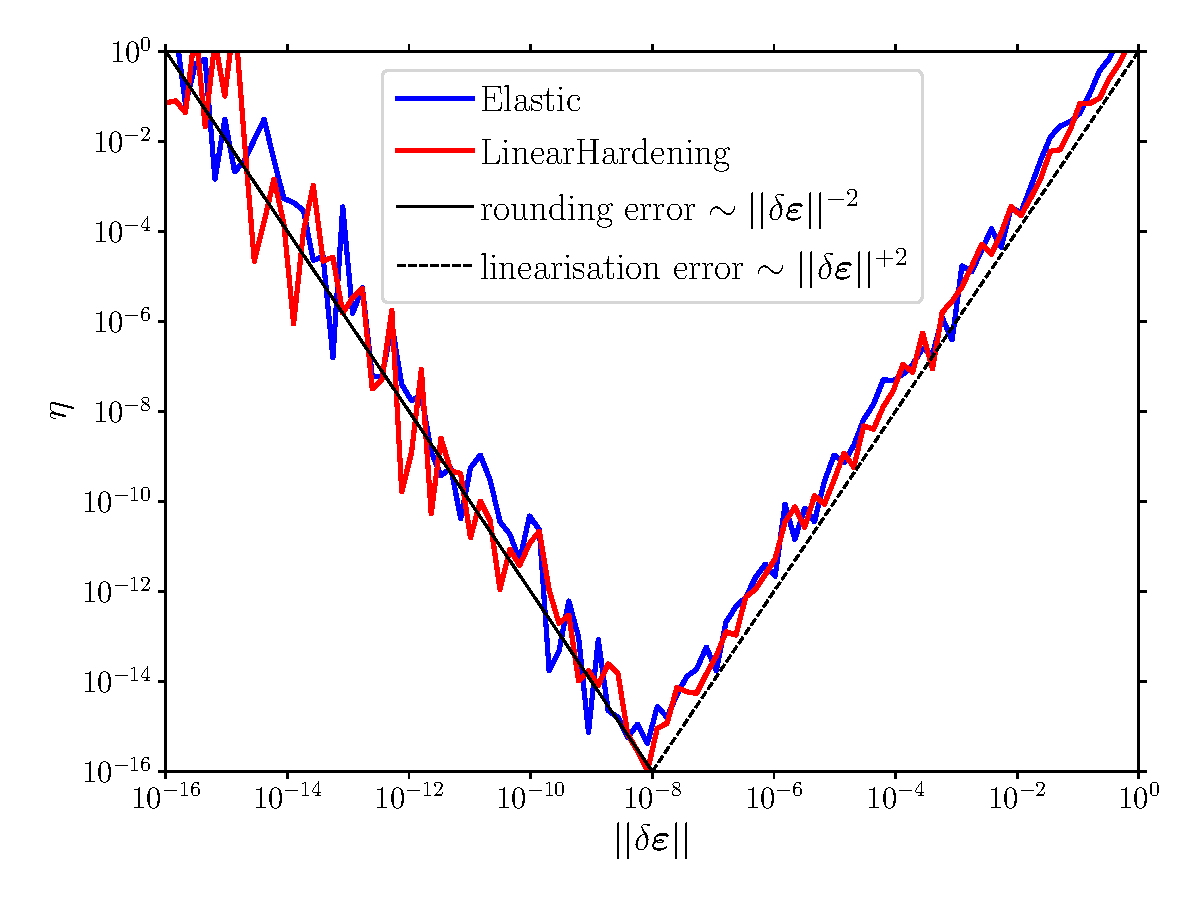
\includegraphics[width=.5\textwidth]{examples/consistency}
    \caption{
        Result of the consistency check
        (performed in the reference configuration, as in \cref{eq:tangent:ref}).}
    \label{fig:consistency}
\end{figure}

\bibliography{library}

\end{document}
